\documentclass[dvipdfmx]{jsarticle}
\usepackage{tikz}
\usetikzlibrary{arrows}
\usetikzlibrary{patterns}
\usepackage{amsmath}
\begin{document}

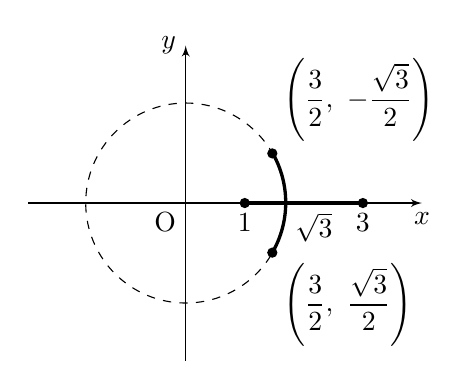
\begin{tikzpicture}[ > = latex']

         \node(O) at (0,0) [below left]{$\mathrm{O}$};
         \draw[->] (-2,0) -- (3,0) node[below]{$x$};
         \draw[->] (0,-2) -- (0,2) node[left]{$y$};
         \draw[dashed](0,0)circle[radius=1.27];
         \draw[very thick](1.1, - 0.63) node[below right]{$\left(\dfrac{3}{2},\  \dfrac{\sqrt{3} }{2}\right)$} arc(-30:30:1.27) node[above right]{$\left(\dfrac{3}{2},\ - \dfrac{\sqrt{3} }{2}\right)$};
         \node[draw, circle, thick, fill, minimum size=1mm, inner sep=0] at (1.1, - 0.63) {};
         \node[draw, circle, thick, fill, minimum size=1mm, inner sep=0] at (1.1,  0.63) {};
         \draw[very thick] (0.75,0) node[below]{$1$} -- (2.25,0) node[below]{$3$};
         \draw (1.27,0) node [below right] {$\sqrt{3}$};
         \node[draw, circle, thick, fill, minimum size=1mm, inner sep=0] at (0.75,0) {};
         \node[draw, circle, thick, fill, minimum size=1mm, inner sep=0] at (2.25,0) {};


\end{tikzpicture}

        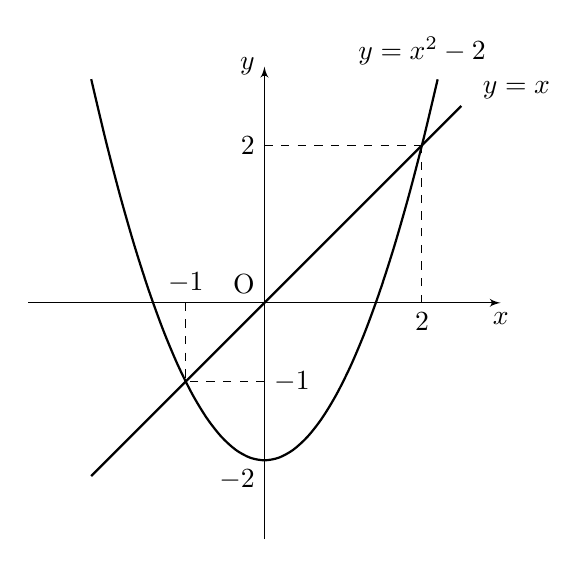
\begin{tikzpicture}[>= latex']
         \draw (0,0) node[above left]{O};
         \draw[->] (-3,0) -- (3,0) node[below]{$x$};
         \draw[->] (0,-3) -- (0,3) node[left]{$y$};
         \draw[thick, domain=-2.2:2.5] plot (\x,\x) node at(3.2,2.7) {$y = x$};
         \draw[thick, domain=-2.2:2.2,smooth] plot (\x,{\x * \x - 2}) node at(2,3.2) {$y = x^2 -  2$};
         \draw[thin,dashed](2,0) node [below]{$2$}--(2,2);
         \draw[thin,dashed](0,2) node [left]{$2$}--(2,2);
         \draw[thin,dashed](-1,0) node [above]{$ -1$}--(-1, -1);
         \draw[thin,dashed](0, -1) node [right]{$ -1$}--( -1, -1);
         \draw (0, -2) node [below left]{$ -2$};
        \end{tikzpicture}
        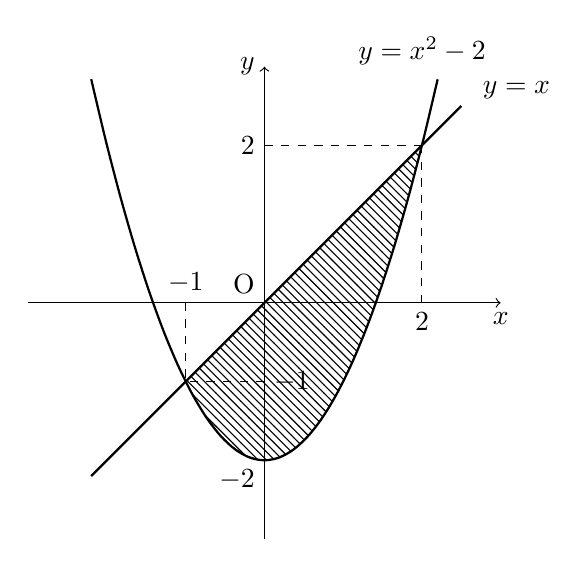
\begin{tikzpicture}
         \draw (0,0) node[above left]{O};
         \draw[->] (-3,0) -- (3,0) node[below]{$x$};
         \draw[->] (0,-3) -- (0,3) node[left]{$y$};
         data{
         x,y
         - 2.5, - 2.5
         2.5, 2.5
         };
         \begin{scope}
          \draw[thick, domain=-2.2:2.5] plot (\x,\x) node at(3.2,2.7) {$y = x$};
          \draw[thick, domain=-2.2:2.2,smooth] plot (\x,{\x * \x - 2}) node at(2,3.2) {$y = x^2 -  2$};
          \draw[thin,dashed](2,0) node [below]{$2$}--(2,2);
          \draw[thin,dashed](0,2) node [left]{$2$}--(2,2);
          \draw[thin,dashed](-1,0) node [above]{$ -1$}--(-1, -1);
          \draw[thin,dashed](0, -1) node [right]{$ -1$}--( -1, -1);
          \draw (0, -2) node [below left]{$ -2$};
          \clip (-2.5,-2.5) |- (0, - 2.5) -| (2.5,2.5) --cycle;
          \clip [draw,domain= -2:2.2] plot (\x,{\x * \x - 2});
          \draw [pattern=north west lines](-2.5, -2.5) rectangle (2.5,2.5);
         \end{scope}
        \end{tikzpicture}

        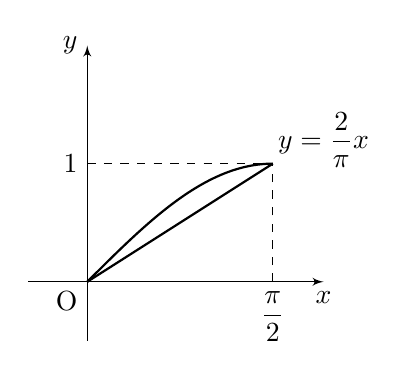
\begin{tikzpicture}[>= latex',scale = 1.5]
         \draw (0,0) node[below left]{O};
         \draw[->] (-0.5,0) -- (2,0) node[below]{$x$};
         \draw[->] (0,-0.5) -- (0,2) node[left]{$y$};
         data{
         x,y
         - 0.5, - 0.5
         2, 1.5
         };
         \draw[thick, domain=-0:pi/2] plot (\x,{(2/pi) * \x}) node at(2,1.2) {$y = \dfrac{2}{\pi}x$};
         \draw[thick] (0, 0) sin (pi/2,1);
         \draw[thin,dashed](pi/2,0) node [below]{$\dfrac{\pi}{2}$}--(pi/2,1);
         \draw[thin,dashed](0,1) node [left]{$1$}--(pi/2,1);
        \end{tikzpicture}

\end{document}